\documentclass[a4paper, 12pt, titlepage]{report}
\usepackage{amsmath, amssymb}
\usepackage{graphicx}
\usepackage{caption}
\usepackage{appendix}
\usepackage{chngcntr}
\usepackage{hyperref}
\usepackage{multirow}
\usepackage[left=20mm,right=20mm,top=15mm,bottom=15mm]{geometry}
\usepackage[backend=biber]{biblatex}
\addbibresource{references.bib}

\counterwithout{figure}{chapter}
\counterwithout{table}{chapter}
\counterwithout{equation}{chapter}

\begin{document}
\title{EE466: Power Electronics, Machines and Applications Coursework 2}
\author{Scott McBride}
\date{\today}
\maketitle
\tableofcontents
\chapter{Introduction}
This coursework submission shows the worked solutions for part 2 of the coursework assessment. Each question within this corresponds to the relevant question from the coursework specification. Where necessary, additional context is provided to clarify any assumptions within the design processes along with any relevant information provided within the brief.

All relevant files for this submission are contained within the GitHub Repository at this \href{https://github.com/WithASideOfSalt/EE466-Coursework-2}{link}.

\chapter{Question 1}
\section{Context}
This question looks at the Thermal energy transfer between 2 heat sources contained within the same system. Contained within Table~\ref{tab:question1} are the relevant parameters for the system, those being the IGBT, Diode, heatsink and ambient temperature provided by~\cite{EE466CourseworkPart2}

\begin{table}[htbp]
    \centering
    \caption{Parameters for Question 1}
    \label{tab:question1}
    \begin{tabular}{|c|c|c|}
        \hline
        \textbf{Component} & \textbf{Parameter} & \textbf{Value} \\
        \hline
        \multirow{3}{*}{IGBT}
        & Power Dissipation \(W_{\mathrm{IGBT}}\) & 12 W \\
        & Junction-to-case thermal resistance \(R_{\theta jc}\) & \(0.6\,^\circ\mathrm{C/W}\) \\
        & Case-to-heatsink thermal resistance \(R_{\theta chs}\) & \(1.4\,^\circ\mathrm{C/W}\) \\
        \hline
        \multirow{3}{*}{Diode}
        & Power Dissipation \(W_{\mathrm{Diode}}\) & 7 W \\
        & Junction-to-case thermal resistance \(R_{\theta jc}\) & \(0.9\,^\circ\mathrm{C/W}\) \\
        & Case-to-heatsink thermal resistance \(R_{\theta chs}\) & \(1.5\,^\circ\mathrm{C/W}\) \\
        \hline
        \multirow{3}{*}{Heatsink}
        & Heatsink-to-ambient thermal resistance \(R_{\theta hsa}\) & \(3.2\,^\circ\mathrm{C/W}\) \\
        & Thermal capacitance \(C_{\theta hs}\) & \(280\,\mathrm{J/^\circ C}\) \\
        & Ambient temperature & \(40\,^\circ\mathrm{C}\) \\
        \hline
    \end{tabular}
\end{table}

\section{1a}
\begin{figure}[!h]
    \centering
    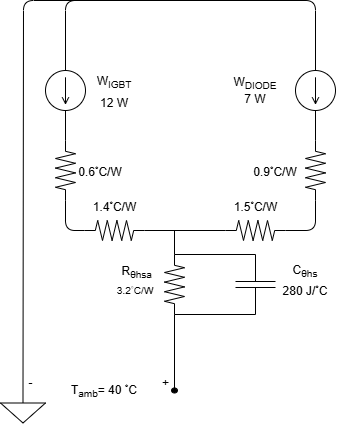
\includegraphics[width=0.3\textwidth]{./Images/Q1Ai.png}
    \caption{Thermal Equivalent Circuit for Question 1a}
    \label{fig:question1a}
\end{figure}
\section{1b}
\chapter{Question 2}
\section{Context}
\section{2a}
\section{2b}
\section{2c}
\chapter{Question 3}
\section{Context}
\section{3a}
\section{3b}
\section{3c}

\printbibliography

\end{document}